%20 min preso!
\documentclass[xcolor=table,english]{beamer}
\usepackage{beamerthemesplit}
\usepackage{wrapfig}
\usetheme{SPbGU}
\usepackage{pdfpages}
\usepackage{amsmath}
\usepackage{mathtools}
\usepackage{cmap}
\usepackage{subcaption}
\usepackage[utf8]{inputenc}
\usepackage[T1, T2A]{fontenc}
\usepackage[]{babel}
\usepackage{indentfirst}
\usepackage{amsmath}
\usepackage{tikz}
\usepackage{multirow}
\usepackage[noend]{algpseudocode}
\usepackage{algorithm}
\usepackage{algorithmicx}
\usepackage{fancyvrb}
\usetikzlibrary{calc}
\usetikzlibrary{shapes,arrows}
\usetikzlibrary{arrows,automata}
\usetikzlibrary{positioning}
\usetikzlibrary{fit}

\usepackage{kbordermatrix} % include package @ document preamble
\renewcommand{\kbldelim}{(} % change default array delimiters to parentheses
\renewcommand{\kbrdelim}{)}

\newcommand\mca{\multicolumn{1}{c}{\cellcolor{red}\textbf{\{a\}}}}
\newcommand\mcb{\multicolumn{1}{c}{\cellcolor{red}\textbf{\{b\}}}}

\usepackage{tabularx}
\newcolumntype{Y}{>{\raggedleft\arraybackslash}X}

\renewcommand{\thealgorithm}{}

\newtheorem{mytheorem}{Theorem}
\renewcommand{\thealgorithm}{}

\newcommand{\tikzmark}[1]{\tikz[overlay,remember picture] \node (#1) {};}
\def\Put(#1,#2)#3{\leavevmode\makebox(0,0){\put(#1,#2){#3}}}

\newcommand{\ltz}{$< 1$}


\tikzset{
    state/.style={
           rectangle,
           rounded corners,
           draw=black, very thick,
           minimum height=2em,
           inner sep=2pt,
           text centered,
           },
}

\beamertemplatenavigationsymbolsempty

\title[Flow2Vec]{Flow2Vec: Value-Flow-Based Precise Code Embedding}
\subtitle[YaccConstructor]{Applications of CFPQ analysis}
% То, что в квадратных скобках, отображается в левом нижнем углу.
\institute[СПбГУ]{
JetBrains Research, Лаборатория языковых инструментов  \\
Санкт-Петербургский Государственный университет
}

% То, что в квадратных скобках, отображается в левом нижнем углу (прикольно).
\author[Егор Орачев]{\textbf{Егор Орачев}}
\date{22 марта 2021}


\begin{document}
{
\begin{frame}[fragile]
  \begin{table}
  \centering
  \begin{tabularx}{\linewidth}{YcX}
    
\includegraphics[height=1.5cm]{pictures/jetbrainsResearch.pdf} \hfill
    & \begin{minipage}[t]{0.3\textwidth}\center \vspace{-1cm}  Семинар
      \end{minipage}
    & \hfill 
\includegraphics[height=1.5cm]{pictures/SPbGU_Logo.png}
  \end{tabularx}
  \end{table}
  \titlepage
\end{frame}
}

\begin{frame}[fragile] \frametitle{Предметная область}
    \begin{minipage}[m]{0.45\linewidth}
        \begin{figure}
            \centering
            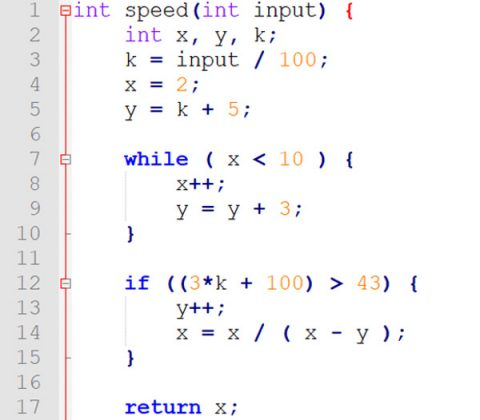
\includegraphics[width=0.8\textwidth]{figures/static_code_analysis.jpg}
            \caption{Code fragment}
            \label{fig:code_fragment}
        \end{figure}
    \end{minipage}\hfill
    \begin{minipage}[m]{0.55\linewidth}
        \textbf{Статический анализ кода}
        \begin{itemize}
            \item Interprocedural data flow analysis
            \item Program slicing
            \item Pointer  analysis
            \item Shape analysis
            \item Code classification
            \item Code summarization
        \end{itemize}
    \end{minipage}
\end{frame}

\begin{frame}[fragile] \frametitle{Представление программы}
    \begin{itemize}
        \item Проблема: эффективность анализа зависит от того, насколько "хорошим" является используемое представление программы
        \item Варианты: 
        {
            \begin{itemize}
                \item Абстрактное синтаксическое дерево
                \item Представление в промежуточном языке
                \item Граф потока данных
                \item Граф потока управления
                \item Граф вызовов
                \item Представление программы в виде embedding'а
            \end{itemize}
        }
    \end{itemize}
\end{frame}

\begin{frame}[fragile] \frametitle{Структура презентации}
    \begin{itemize}
        \item Code2vec: метод и его описание
        \item Построение embedding'а для ориентированного графа
        \item Запросы с контекстно-свободными (КС) ограничениями
        \item Flow2vec: метод и его описание
        \item Flow2vec: практическое применение
        \item Наши исследования в области вычисления КС запросов
        \item Дальнейшее направление исследований  
    \end{itemize}
\end{frame}

\begin{frame}[fragile] \frametitle{Code2vec: Code Embedding}
    \begin{itemize}
        \item Code2vec\footnote{Code2vec: learning distributed representations of code, Uri Alon, Meital Zilberstein, Omer Levy, and Eran Yahav, \href{https://doi.org/10.1145/3290353}{https://doi.org/10.1145/3290353}}: построение code embeddings для представление фрагментов кода 
        в виде числовых векторов фиксированной длины
        \item Идея:
        {
            \begin{enumerate}
                \item Представить фрагмент кода в виде абстрактного ситнаксического дерева
                \item Сделать случайную выборку путей из дерева
                \item Получить векторное представление путей
                \item Суммировать полученные представления с весами и получить финальный вектор
                \item Использовать данный вектор для анализа программы
                \item Выполнять шаги 3 и 4 одновременно 
            \end{enumerate}
        }
    \end{itemize}
\end{frame}

\begin{frame}[fragile] \frametitle{Code2vec: Мотивационный пример}
    \begin{minipage}[m]{\linewidth}
        \begin{figure}
            \centering
            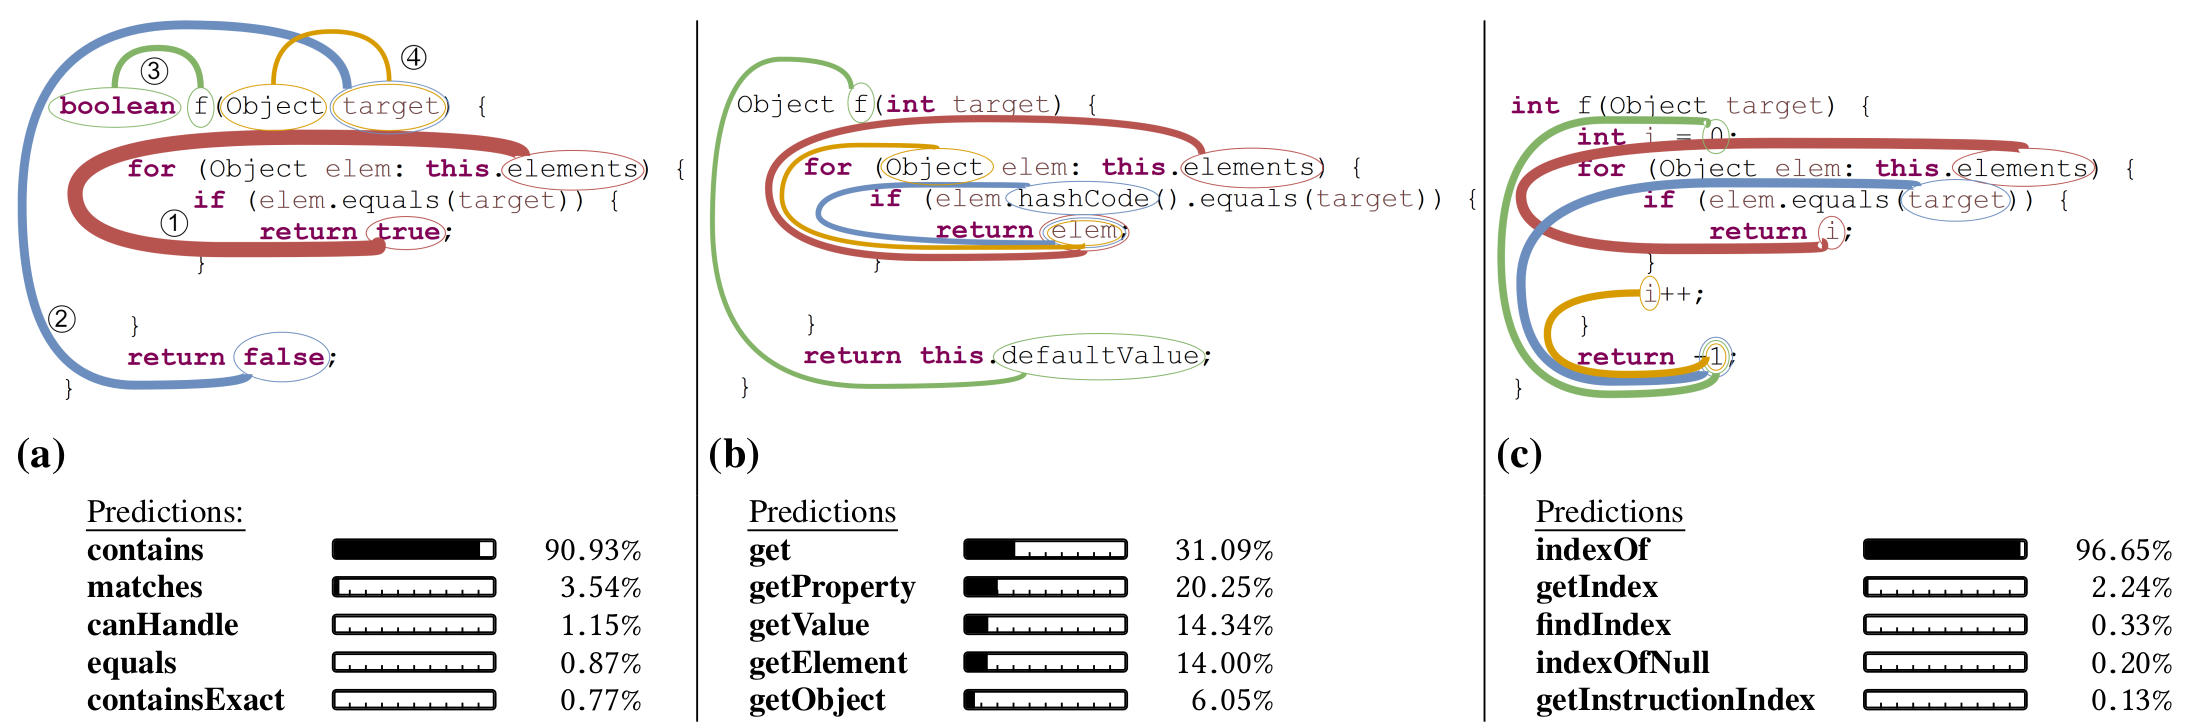
\includegraphics[width=\textwidth]{figures/code2vec_motivation_example.png}
            \caption{An example for three methods that albeit having have a similar syntactic structure can be easily distinguished by our model; our model successfully captures the subtle differences between them and manages to predict meaningful names. Each method portrays the top-4 paths that were given the most attention by the model. The widths of the colored paths are proportional to the attention that each path was given.}
        \end{figure}
    \end{minipage}\hfill
\end{frame}

\begin{frame}[fragile] \frametitle{Code2vec: Терминология}
    \begin{itemize}
        \item  Абстрактное синтаксическое дерево (АСТ) $\mathcal{C} = \langle N, T, X, s, \delta, \phi \rangle$, $\delta : N \rightarrow (N \cup T)^*$, $\phi : T \rightarrow X$
        \item Путь в дереве $p = n_1 d_1 ... n_k d_k n_{k+1}$, $n_1, n_{k+1} \in T$, $n_2, ..., n_k \in N$, $d_i \in \{ \uparrow, \downarrow \}$
        \item Путь-контекст $\langle x_s, p, x_t \rangle$, $x_s, x_t \in X$, $x_s = \phi(start(p))$, $x_t = \phi(end(p))$, для \textit{$x = 7$} путь-контекст $\langle x, NameExpr \uparrow AssignExpr \downarrow IntegerLiteralExpr, 7\rangle$
        \item Множество меток Y, P множество АСТ путей, извлекаемых из датасета
    \end{itemize}
\end{frame}

\begin{frame}[fragile] \frametitle{Code2vec: Модель (1)}
    \begin{itemize}
        \item Что будем обучать:
        {
            \begin{itemize}
                \item embedding путей $path\_vocab \in \mathbb{R}^{|P| \times d}$
                \item embedding значений $value\_vocab \in \mathbb{R}^{|X| \times d}$
                \item полносвязный слой $W \in \mathbb{R}^{d \times 3d}$
                \item вектор внимания $\textbf{a} \in \mathbb{R}^d$
                \item embedding меток $tags\_vocab \in \mathbb{R}^{|Y| \times d}$
            \end{itemize}
        }
        \item Параметр $d \in \mathbb{N}$ - размерность embedding'а, подбирается эмпирически
    \end{itemize}
\end{frame}

\begin{frame}[fragile] \frametitle{Code2vec: Модель (2)}
    \begin{minipage}[m]{\linewidth}
        \begin{figure}
            \centering
            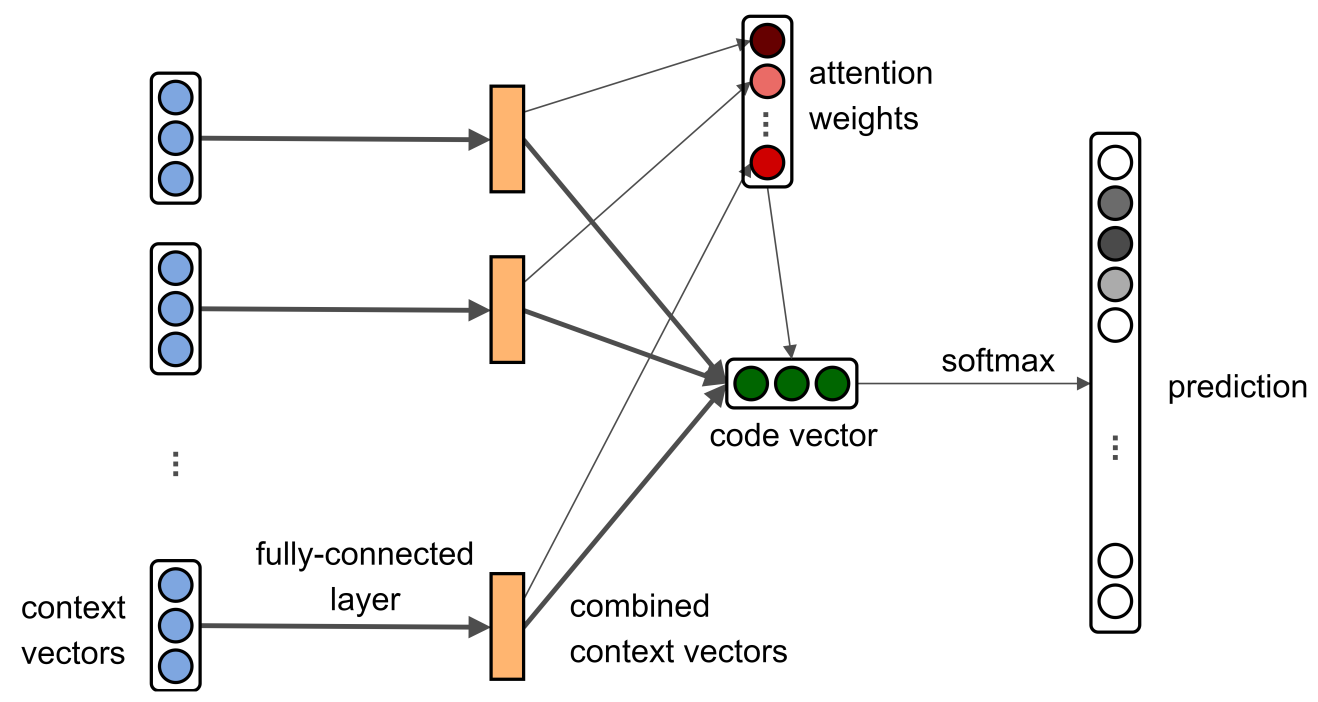
\includegraphics[width=0.8\textwidth]{figures/code2vec_model.png}
            \caption{The architecture of our path-attention network. A full-connected layer learns to combine embeddings of each path-contexts with itself; attention weights are learned using the combined context vectors, and used to compute a code vector. The code vector is used to predicts the label.}
        \end{figure}
    \end{minipage}\hfill
\end{frame}

\begin{frame}[fragile] \frametitle{Code2vec: Code as Bag of Path-Contexts}
    \begin{itemize}
        \item Множество всех путей P
        \item Фрагмент кода $C = \langle N, T, X, s, \delta, \phi \rangle$
        \item $T_{pairs} = \{ (t_i, t_j)~|~t_i, t_j \in termNodes(C), i \neq j\}$
        \item $Rep = \{ \langle x_s, p, x_t \rangle ~|~ p \in P$ и $\exists (t_i, t_j) \in T_{pairs}:$ $start(p) = x_s, end(p) = x_t$, где $x_s = \phi(t_i), x_t = \phi(t_j) \}$
        \item Мешок путей-контекстов $\mathcal{B} = \{ b_1, ... , b_n \}$, $b_i \in Rep$
    \end{itemize}
\end{frame}

\begin{frame}[fragile] \frametitle{Code2vec: Path-Attention Model}
    \begin{itemize}
        \item Контекстный вектор $c_i = embedding(\langle x_s, p_j, x_t \rangle) = [value\_vocab_s, path\_vocab_j, value\_vocab_t] \in \mathbb{R}^{3d}$
        \item Комбинированный контекстный вектор $\tilde{c_i} = tanh(W * c_i) \in \mathbb{R}^d$
        \item Веса внимания $\alpha_i = \frac{exp({c_i}^T \cdot \textbf{a})}{\Sigma_{j=1}^n exp({c_j}^T \cdot \textbf{a})}$
        \item Вектор фрагмента кода $\textbf{v} = \Sigma_{i=1}^n \alpha_i \tilde{c_i}$
        \item Предсказание $y_i \in Y, q(y) = \frac{exp(\textbf{v}^T \cdot \textit{tags\_vocab}_i)}{\Sigma_{i=1}^{|Y|} exp(\textbf{v}^T \cdot \textit{tags\_vocab}_j) }$
    \end{itemize}
\end{frame}

\begin{frame}[fragile] \frametitle{Code2vec: Резюме}
    \begin{itemize}
        \item Можем представить пути в АСТ дереве фрагмента кода в виде набора векторов
        \item Используя взвешенную сумму, можем представить весь фрагмент кода как вектор
        \item Полученный вектор можем использовать в дальнейшем для анализа
    \end{itemize}
\end{frame}

\begin{frame}[fragile] \frametitle{HOPE: Graph Embedding}
    \begin{itemize}
        \item Построение представления графа в векторном пространстве выбранной размерности
        {
            \begin{itemize}
                \item Вершины графа --- это вектора
                \item Можно использовать в задачах реконтсрукции графа, рекомендации соседей, предстказания связей и т.д.
            \end{itemize} 
        }
        \item Проблемы:
        {
            \begin{itemize}
                \item Необходимо сохранить "важные" свойства графа
                \item Реальные графы является ориентированными и обладают ассиметричной транзитивностью
            \end{itemize}
        }
        \item Решение: Алгоритм High-Order Proximity preserved Embedding (HOPE)\footnote{Asymmetric Transitivity Preserving Graph Embedding, Mingdong Ou, Peng Cui, Jian Pei, Ziwei Zhang, and Wenwu Zhu, \href{https://doi.org/10.1145/2939672.2939751}{https://doi.org/10.1145/2939672.2939751}}
    \end{itemize}
\end{frame}

\begin{frame}[fragile] \frametitle{HOPE: Идея}
    \begin{minipage}[m]{\linewidth}
        \begin{figure}
            \centering
            \begin{subfigure}[b]{0.45\textwidth}
                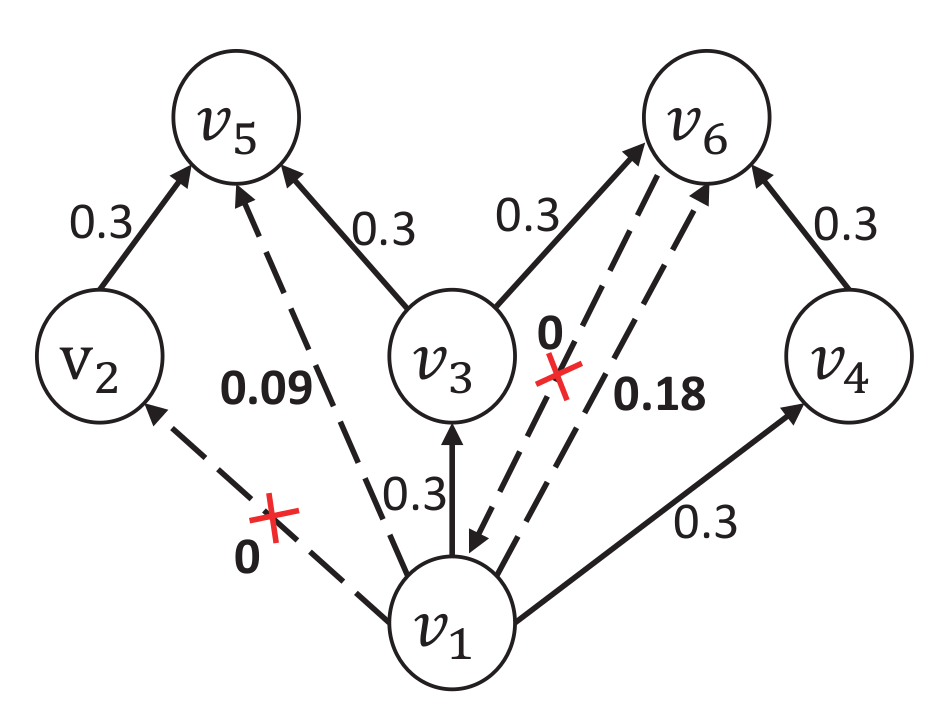
\includegraphics[width=\textwidth]{figures/hope_graph.png}
                \caption{Directed graph}
            \end{subfigure}
            \hfill
            \begin{subfigure}[b]{0.45\textwidth}
                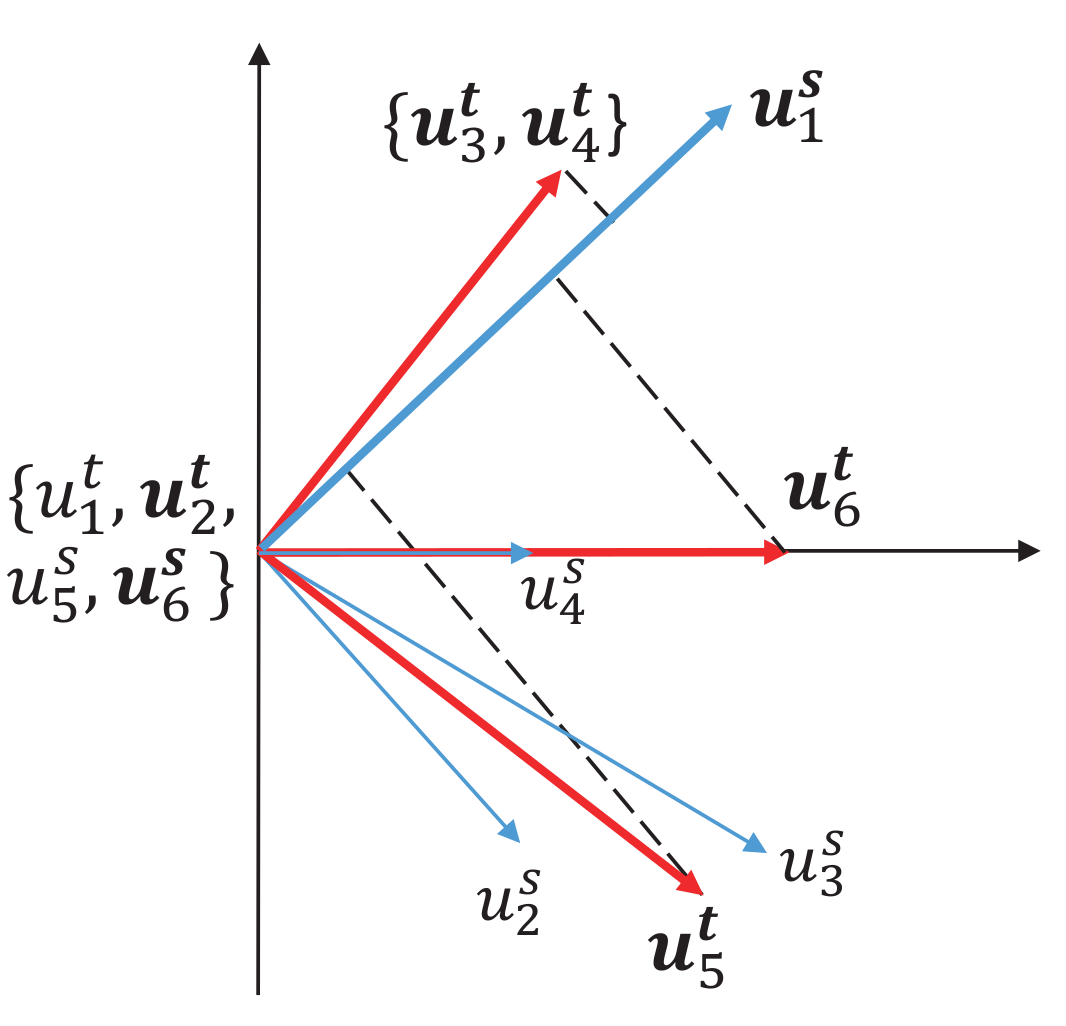
\includegraphics[width=\textwidth]{figures/hope_embedding.png}
                \caption{Graph embedding}
            \end{subfigure}
            \caption{HOPE: Asymmetric Transitivity Preserving Graph Embedding}
        \end{figure}
    \end{minipage}\hfill
\end{frame}

\begin{frame}[fragile] \frametitle{HOPE: Постановка задачи}
    \begin{itemize}
        \item Ориентированный граф $G = \langle V, E \rangle$, $V = \{ v_1, ... , v_N \}$, $|V| = N$, $e_{ij}=(v_1, v_2) \in E$
        \item Матрица смежности графа $A \in \mathbb{R}^{N \times N}$, $a_i$ - i-ая строка матрицы, $A_{ij}$ - элемент матрицы в i-ой строке и j-том столбце
        \item Матрица $S \in \mathbb{R}^{N \times N}$ - матрица близости графа
        \item Embedding матрицы $U = [U^s, U^t]$, $U^s, U^t \in \mathbb{R}^{N \times K}$, $K \in \mathbb{N}$ - размерность emdedding'а, вектора $u^s_i, u^t_i$ соответсвуют вершине графа $v_i$
        \item \textbf{Хотим приблизить матрицу $S$ оптимально в следующем смысле $min \| S - U^s * {U^t}^T \|^2_F$, где $\| \bullet \|_F$ - норма Фробениуса} 
    \end{itemize}
\end{frame}

\begin{frame}[fragile] \frametitle{HOPE: High-order Proximity Matrix}
    \begin{itemize}
        \item Построение матрицы близости $S$, которая сохранит "важные" свойства графа для дальнейшего анализа
        \item Варианты выбора $S$:
        {
            \begin{itemize}
                \item Индекс Катца (англ. Katz index): \\$S^{Katz} = \Sigma_{i=1}^{\infty} \beta^i A^i$, где $\beta \in (0, 1)$ - фактор ослабления
                \item Rooted PageRank
                \item Common Neighbors
                \item Adamic-Adar
            \end{itemize}
        }
        \item Только Katz index и Rooted PageRank сохраняют глобальную ассиметричную транзитивность графа
    \end{itemize}
\end{frame}

\begin{frame}[fragile] \frametitle{HOPE: Approximation of High-Order Proximity}
    \begin{itemize}
        \item $S = S^{Katz} = \Sigma_{i=1}^{\infty} \beta^i A^i$, \\$S^{Katz} = \beta A * S^{Katz} + \beta * A$, $S^{Katz} = (I - \beta A)^{-1} * \beta A$
        \item $S = \Sigma_{i=1}^N \sigma_i v_i^s {v_i^t}^T$ используя SVD разложение, где $\{\sigma_1, ... , \sigma_N\}$ сингулярные значения в порядке убывания
        \item $U^s = [ \sqrt{\sigma_1} * v_1^s, ..., \sqrt{\sigma_K} * v_K^s ]$
        \item $U^t = [ \sqrt{\sigma_1} * v_1^t, ..., \sqrt{\sigma_K} * v_K^t ]$
        \item Ошибка аппроксимации: $\| S - U^s * {U^t}^T \|^2_F = \Sigma_{i=K+1}^N \sigma_i^2$
        \item Относительная ошибка аппроксимации: $\dfrac{\| S - U^s * {U^t}^T \|^2_F}{\| S \|^2_F} = \dfrac{\Sigma_{i=K+1}^N \sigma_i^2}{\Sigma_{i=1}^N \sigma_i^2}$
    \end{itemize}
\end{frame}

\begin{frame}[fragile] \frametitle{HOPE: Резюме}
    \begin{itemize}
        \item Для ориентированного графа $G$ можем построить embedding, который сохраняет ассиметричную транзитивность графа
        \item Для построения требуется матрица близости высокого порядка $S$, которая сохраняет 
        глобальную ассиметричную транзитивность графа
        \item Полученный embedding $U = [U^s, U^t]$ обладает имеет доказанные оценками ошибки приближения. Значение ошибки можно уменьшить, увеличив значение параметра $K$
    \end{itemize}
\end{frame}

\begin{frame}[fragile] \frametitle{Context-free Path Querying}
    \begin{minipage}[m]{0.45\linewidth}
        \begin{figure}
            \centering
            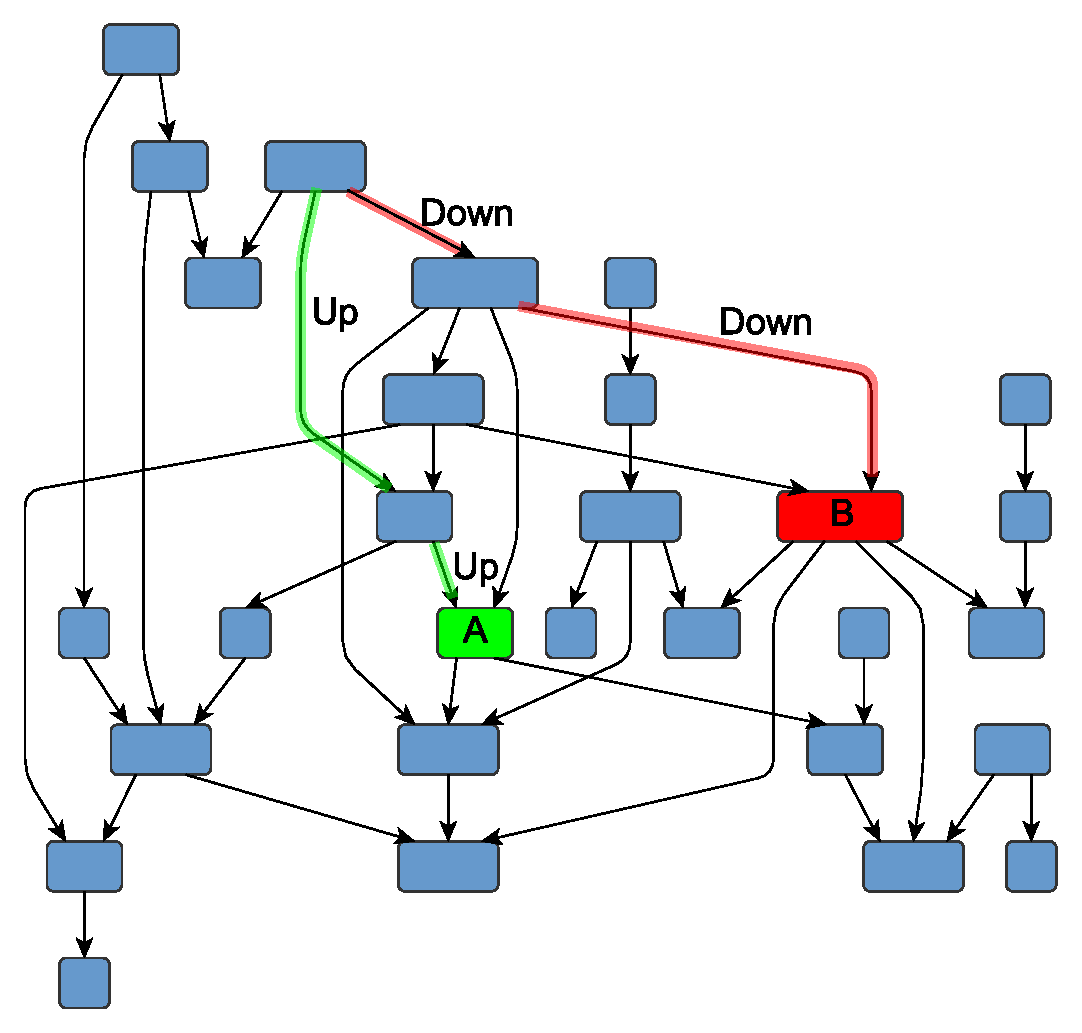
\includegraphics[width=0.8\textwidth]{pictures/hierarchical.pdf}
            \caption{Example of a graph}
        \end{figure}
    \end{minipage}\hfill
    \begin{minipage}[m]{0.55\linewidth}
        \textbf{Навигация в графе:}
        \begin{itemize}
            \item Находятся ли вершины A и B на одном уровне иерархии?
            \item Существует ли путь вида $\textbf{Up}^n \, \textbf{Down}^n$?
            \item Найти все такие пути $\textbf{Up}^n \, \textbf{Down}^n$, которые начинаются в вершине~А
        \end{itemize}
    \end{minipage}
\end{frame}

\begin{frame}[fragile] \frametitle{Context-free Path Querying: Применение}
    \begin{itemize}
        \item Графовые базы данных\footnote{Querying Graph Databases, Pablo Barceló Baeza,  \href{https://doi.org/10.1145/2463664.2465216}{https://doi.org/10.1145/2463664.2465216}}
        \item Анализ RDF данных\footnote{Context-Free Path Queries on RDF Graphs, Xiaowang Zhang, Zhiyong Feng, Xin Wang et al., \href{https://arxiv.org/abs/1506.00743}{https://arxiv.org/abs/1506.00743}}
        \item Биоинформатика\footnote{Quantifying variances in comparative RNA secondary structure prediction, James Anderson, Adám Novák, Zsuzsanna Sükösd et al., \href{https://bmcbioinformatics.biomedcentral.com/articles/10.1186/1471-2105-14-149}{https://bmcbioinformatics.biomedcentral.com/articles/10.1186/1471-2105-14-149}}
        \item Статический анализ кода\footnote{Fast Algorithms for Dyck-CFL-Reachability with Applications to Alias Analysis, Qirun Zhang, Michael R. Lyu, Hao Yuan, Zhendong Su, \href{https://doi.org/10.1145/2499370.2462159}{https://doi.org/10.1145/2499370.2462159}}
    \end{itemize}
\end{frame}

\begin{frame}[fragile] \frametitle{Context-free Path Querying: Терминология}
    \begin{itemize}
        \item Ориентированный граф с меткаи $\mathcal{G} = \langle V, E, L \rangle$
        \item $\omega(\pi) = \omega(v_0 \xrightarrow{l_0} v_1 \xrightarrow{l_1} \cdots \xrightarrow{l_{n-2}} v_{n-1} \xrightarrow{l_{n-1}} v_n) = l_0 l_1 \cdots l_{n-1}$
        \item КС Грамматика $G = \langle \Sigma, N, P, S \rangle$
        \item Язык $L(G) = \{ w~|~S \rightarrow^*_G w \}$
        \item Семантика достижимости: $R = \{ (u, v) ~|~ \exists u \pi v: \omega(\pi) \in L \}$
        \item Семантика всех путей: $\Pi = \{ u \pi v ~|~ \omega(\pi) \in L \}$
    \end{itemize}
\end{frame}

\begin{frame}[fragile] \frametitle{Context-free Path Querying: Пример}
    \begin{minipage}[m]{\linewidth}
        \begin{figure}
            \centering
            \begin{subfigure}[b]{0.35\textwidth}
                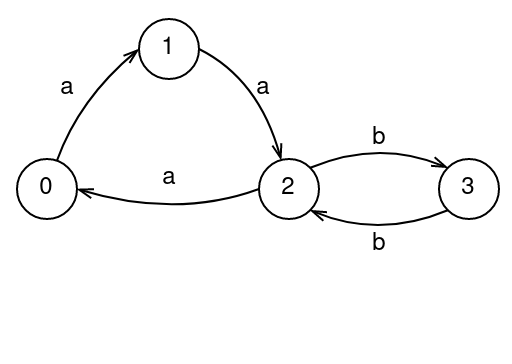
\includegraphics[width=\textwidth]{figures/graph_cfpq_1.png}
                \caption{Input graph}
            \end{subfigure}
            \hfill
            \begin{subfigure}[b]{0.35\textwidth}
                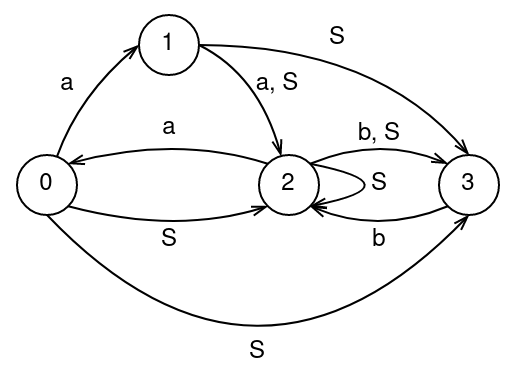
\includegraphics[width=\textwidth]{figures/graph_cfpq_2.png}
                \caption{Result graph}
            \end{subfigure}
            \caption{CFPQ Example}
        \end{figure}
    \end{minipage}\hfill
    \begin{minipage}[m]{\linewidth}
        \begin{itemize}
            \item Грамматика $S \rightarrow aSb~|~ab$
            \item Резульат (Семантика достижимости): ребра с меткой S
            \item Резульат (Семантика всех путей): $\{1 \xrightarrow{a} 3, 0 \xrightarrow{a} 1 \xrightarrow{a} 2 \xrightarrow{b} 3 \xrightarrow{b} 2, 1 \xrightarrow{a} 2 \xrightarrow{a} 0 \xrightarrow{a} 1 \xrightarrow{a} 2 \xrightarrow{b} 3 \xrightarrow{b} 2 \xrightarrow{b} 3 \xrightarrow{b} 2, ...\}$
        \end{itemize}
    \end{minipage}
\end{frame}

\begin{frame}[fragile] \frametitle{Context-free Path Querying: Существующие алгоритмы}
    \begin{itemize}
        \item Алгоритмы, основанные на различных техниках парсинга\\(CYK, LL, LR, etc.)
        \item \textbf{Алгоритмы, основанные на линейной алгебре}
        {
            \begin{itemize}
                \item Матричный алгоритм Рустама Азимова\footnote{Context-Free Path Querying with Single-Path Semantics by Matrix Multiplication, Arseniy Terekhov, Artyom  Khoroshev, Rustam  Azimov, Semyon Grigorev, \href{https://dl.acm.org/doi/10.1145/3398682.3399163}{https://dl.acm.org/doi/10.1145/3398682.3399163}}
                \\- семантика: достижимости, одного пути, всех путей
                \\- платформы: CPU, GPU
                \item Алгоритм на основе пересечения графа и рекурсивного автомата через произведения Кронекера\footnote{Context-Free Path Querying by Kronecker Product, Egor Orachev, Ilya Epelbaum, Rustam  Azimov, Semyon Grigorev, \href{https://link.springer.com/chapter/10.1007/978-3-030-54832-2\_6}{https://link.springer.com/chapter/10.1007/978-3-030-54832-2\_6}}
                \\- семантика: достижимости, одного пути, всех путей
                \\- платформы: CPU, GPU
            \end{itemize}
        }
    \end{itemize}
\end{frame}

\begin{frame}[fragile] \frametitle{Context-free Path Querying: Резюме}
    \begin{itemize}
        \item Для анализа графа можем задавать запросы с КС ограничениями
        \item Для каждой конкретной задачи можем выбирать различную семантику запроса
        \item Имеем ээфективные алгоритмы для вычисления запросов на двух основных вычислительных платформах
    \end{itemize}
\end{frame}

\begin{frame}[fragile] \frametitle{Code Embedding: Проблемы}
    \begin{minipage}[m]{\linewidth}
        \begin{figure}
            \centering
            \begin{subfigure}[b]{0.35\textwidth}
                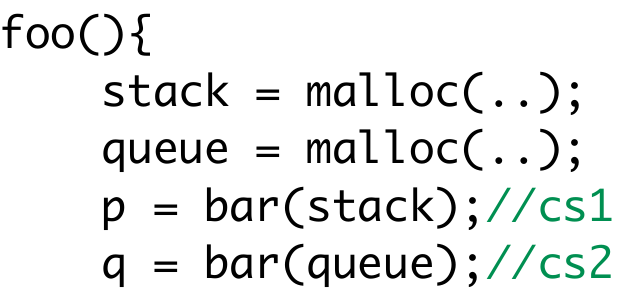
\includegraphics[width=\textwidth]{figures/code_for_ast.png}
                \caption{Foo function}
            \end{subfigure}
            \hfill
            \begin{subfigure}[b]{0.55\textwidth}
                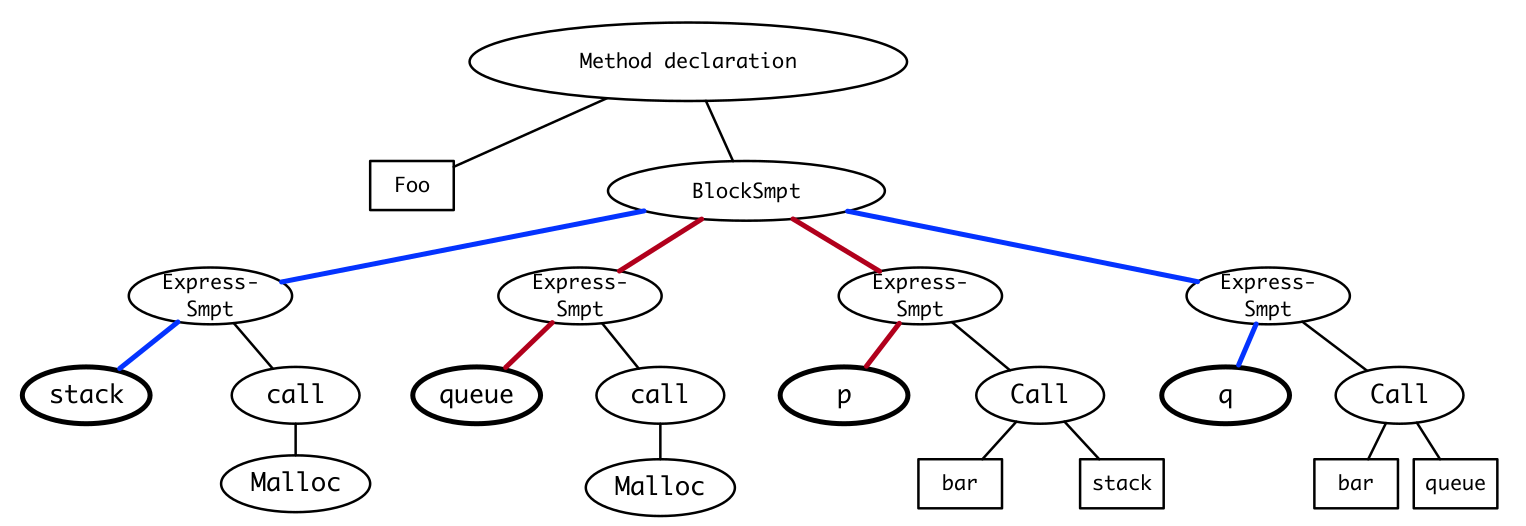
\includegraphics[width=\textwidth]{figures/ast_approach.png}
                \caption{Ast for foo}
            \end{subfigure}
            \caption{Spurious paths example}
        \end{figure}
    \end{minipage}\hfill
    \begin{minipage}[m]{\linewidth}
        Недостатки существующих интсрументов:
        \begin{itemize}
            \item Не учитывют межпроцедурное взаимодействие
            \item Не учитывют псевдонимы (ссылки)
            \item Не учитывют ассиметричную транзитивность программ
        \end{itemize}
    \end{minipage}
\end{frame}

\begin{frame}[fragile] \frametitle{Flow2Vec: Value-Flow-Based Precise Code Embedding}
    \begin{itemize}
            \item Flow2vec\footnote{Flow2Vec: Value-Flow-Based Precise Code Embedding, Yulei Sui, Xiao Cheng, Guanqin Zhang, Haoyu Wang, \href{https://dl.acm.org/doi/10.1145/3428301}{https://dl.acm.org/doi/10.1145/3428301}}: построение code embeddings для представления фрагмента кода как части всей программы с учетом межпроцедурных потоков данных и множества вызовов функций
            \item Идея:
            {
                \begin{enumerate}
                    \item Построить промежуточное представление программы в терминах простых операций
                    \item Построить граф потоков данных
                    \item Используя КС запросы вычислить количество потоков данных между каждым выражение в программе (в ее промежуточном представлении)
                    \item Построить матрицу близости высокого порядка
                    \item Вычислить на ее основе embedding для графа программы
                \end{enumerate}
            }
        \end{itemize}
\end{frame}

\begin{frame}[fragile] \frametitle{Flow2Vec: Обзор}
    \begin{minipage}[m]{\linewidth}
        \begin{figure}
            \centering
            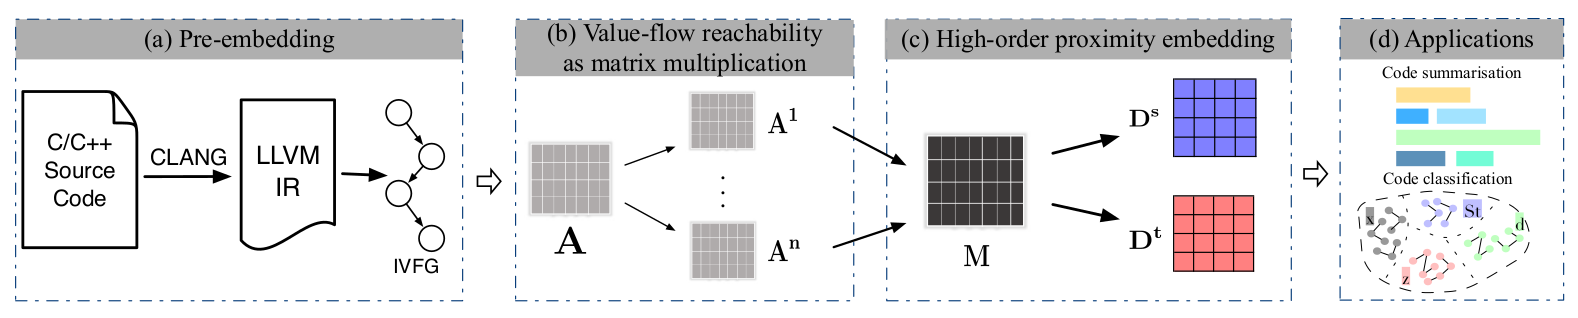
\includegraphics[width=0.9\textwidth]{figures/flow2vec_idea.png}
            \caption{Overview of the approach}
        \end{figure}
    \end{minipage}\hfill
    \begin{minipage}[m]{\linewidth}
        \begin{itemize}
            \item Шаг 1: Построение LLVM-IR, IVFG, исходных матриц с call/return и value-flow информацией
            \item Шаг 2: Value-flow reachability через CFPQ
            \item Шаг 3: Вычисление матрицы близости высокого порядка и построение emdedding'а
            \item Шаг 4: Применение построенного emdedding'а в пользовательских приложениях
        \end{itemize}
    \end{minipage}
\end{frame}

\begin{frame}[fragile] \frametitle{Flow2vec: Pre-embedding (LLVM-IR)}
    \begin{itemize}
        \item LLVM-IR в качестве промежуочного представления
        \item $\mathcal{V} = \mathcal{O} \cup \mathcal{P}$, два типа переменных:
        \\- $\mathcal{O}$ address-taken objects
        \\- $\mathcal{P}$ top-level variables
        \item Конвертация в SSA (Static single assignment form) 
        \item Пять типов инструкций: $p=\&o$, $p=q$, $p=\&q \rightarrow f_i$, $p=*q$, $*p=q$, 
        $p, q \in \mathcal{P}, o \in \mathcal{O}$
    \end{itemize}
\end{frame}

\begin{frame}[fragile] \frametitle{Flow2vec: Pre-embedding (IVFG)}
    \begin{itemize}
        \item Построение  Interprocedural value-flow graph (IVFG) $\langle N, E \rangle$ на основе LLVM-IR программы, где $t \xrightarrow{v} t', v \in \mathcal{V}$ def-use отношение, $t \xrightarrow{p} t', p \in \mathcal{P}$ direct value-flow отношение
        \item Построение
        {
        \begin{enumerate}
            \item Анализ указателей (points-to информация)
            \item Аннотирование: $a = \chi(a)$, $\mu(a)$
            \item Преобразование аннотаций: $a = \chi(a) \implies \textit{def-use}$, $\mu(a) \implies \textit{use}$
            \item Построение def-use цепей для переменных $a \in \mathcal{O}$
        \end{enumerate}
        }
    \end{itemize}
\end{frame}

\begin{frame}[fragile] \frametitle{Flow2vec: Pre-embedding (Example)}
    \begin{minipage}[m]{\linewidth}
        \begin{figure}
            \centering
            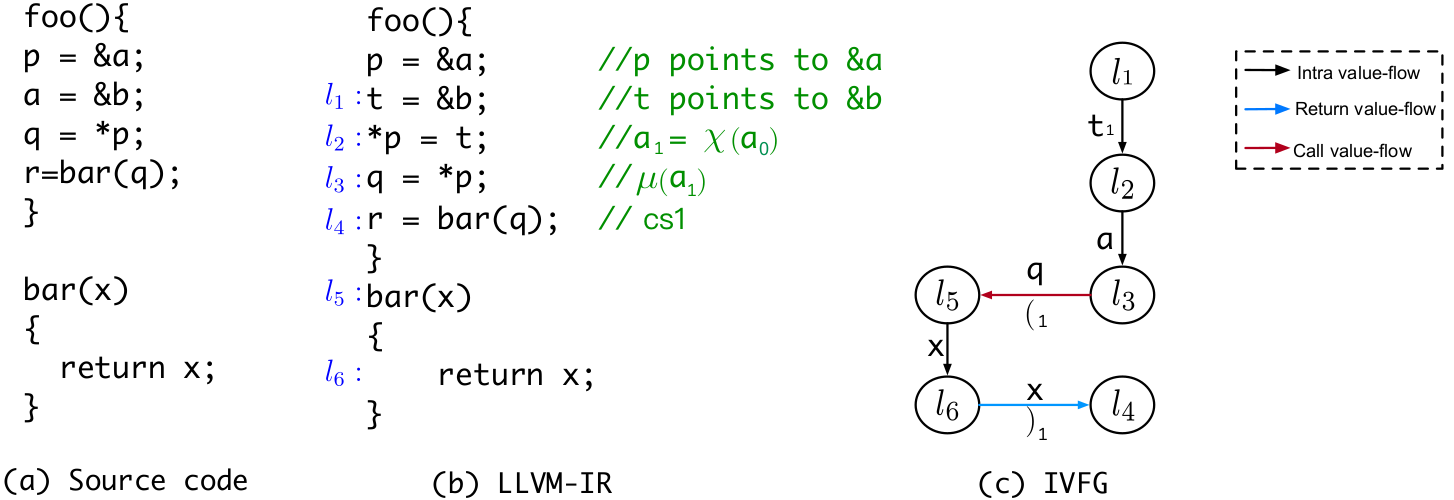
\includegraphics[width=0.9\textwidth]{figures/llvm_ir_and_ivfg.png}
            \caption{A C code fragment and its LLVM instructions and interprocedural value-flow graph (IVFG)}
        \end{figure}
    \end{minipage}\hfill
\end{frame}

\begin{frame}[fragile] \frametitle{Flow2vec: Pre-embedding (Symbolic Matrix)}
    \begin{figure}
        \centering
        \begin{subfigure}[b]{0.45\textwidth}
            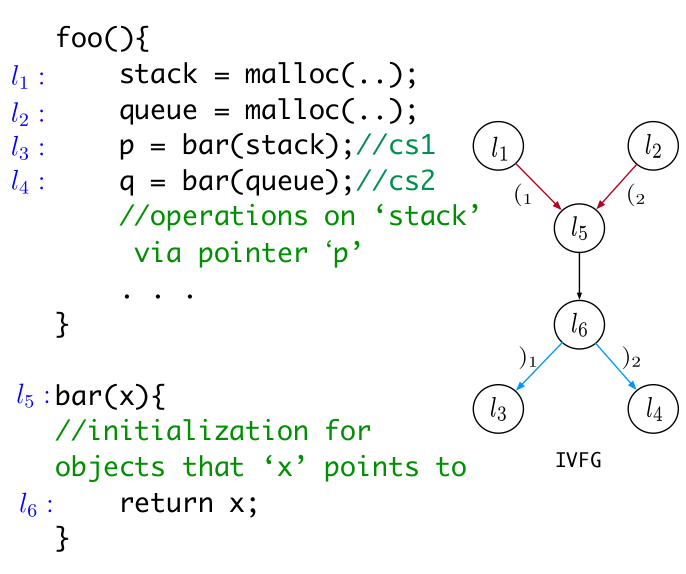
\includegraphics[width=\textwidth]{figures/pre_embeding_a.png}
            \caption{Code fragment and IVFG}
        \end{subfigure}
        \hfill
        \begin{subfigure}[b]{0.45\textwidth}
            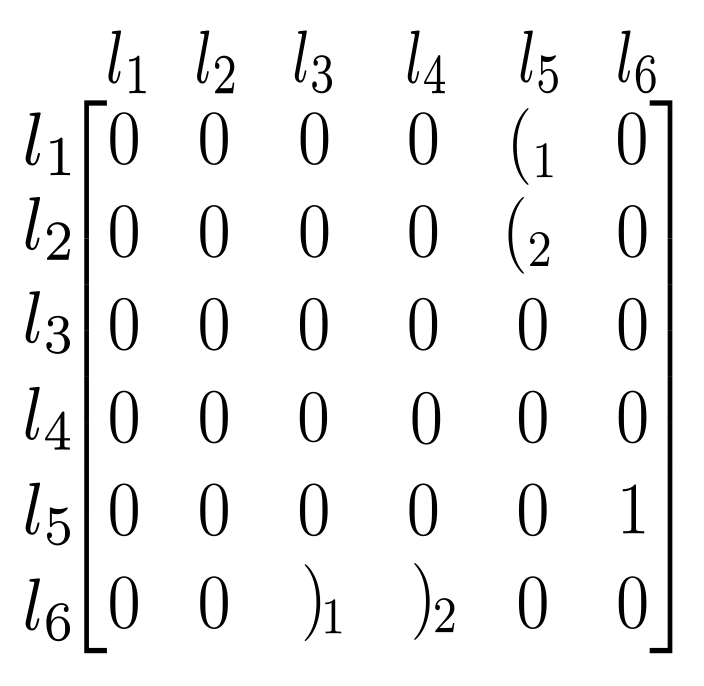
\includegraphics[width=\textwidth]{figures/pre_embedding_b.png}
            \caption{Call/return and value-flow matrix A}
        \end{subfigure}
        \caption{Pre-embedding example. $A_{ij} = 1$ if there is intraprocedural value-flow between $l_i$ and $l_j$. $A_{ij} = (_{csId}$, $A_{ij} = )_{csId}$ for interprocedural value-flow between $l_i$ and $l_j$.}
    \end{figure}
\end{frame}

\begin{frame}[fragile] \frametitle{Flow2vec: Value-flow reachability via matrix multiplication}
    \begin{figure}[w]
        \centering
        \begin{subfigure}[b]{0.2\textwidth}
            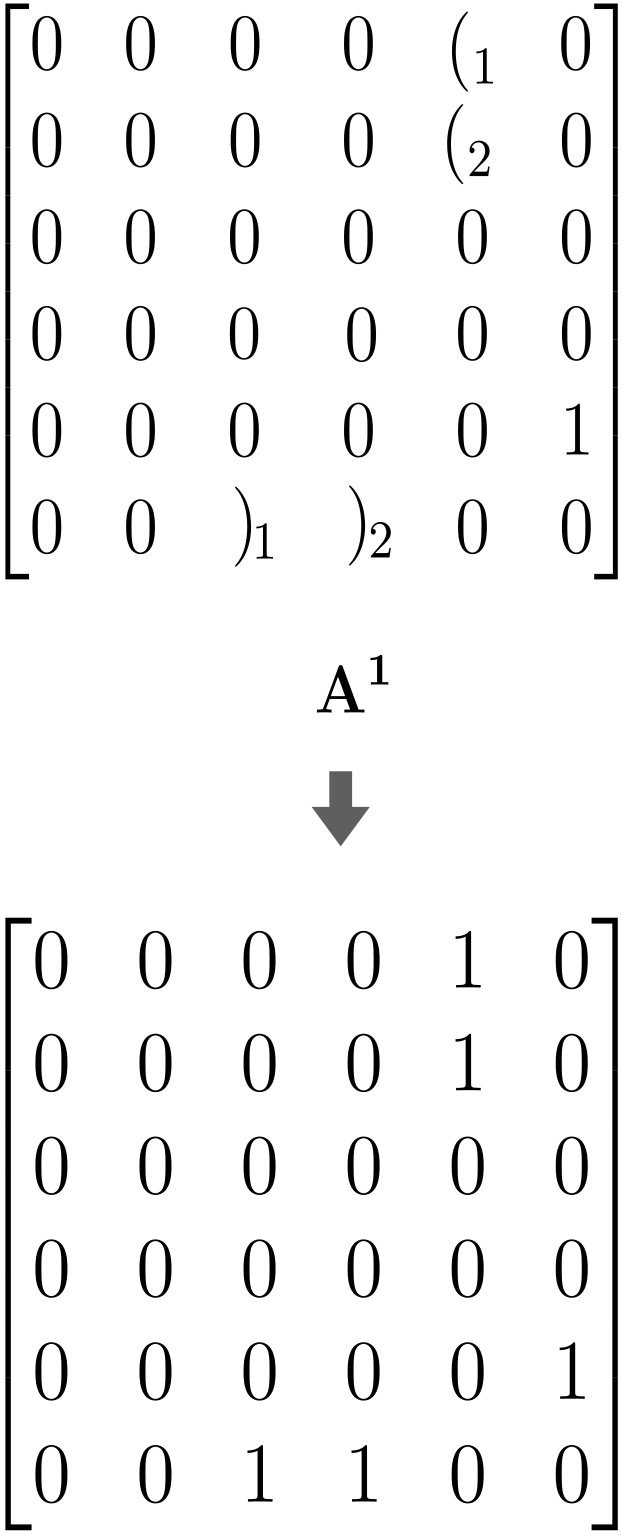
\includegraphics[width=\textwidth]{figures/cfpq_1.png}
            \caption{Matrix $A^1$}
        \end{subfigure}
        \hfill
        \begin{subfigure}[b]{0.268\textwidth}
            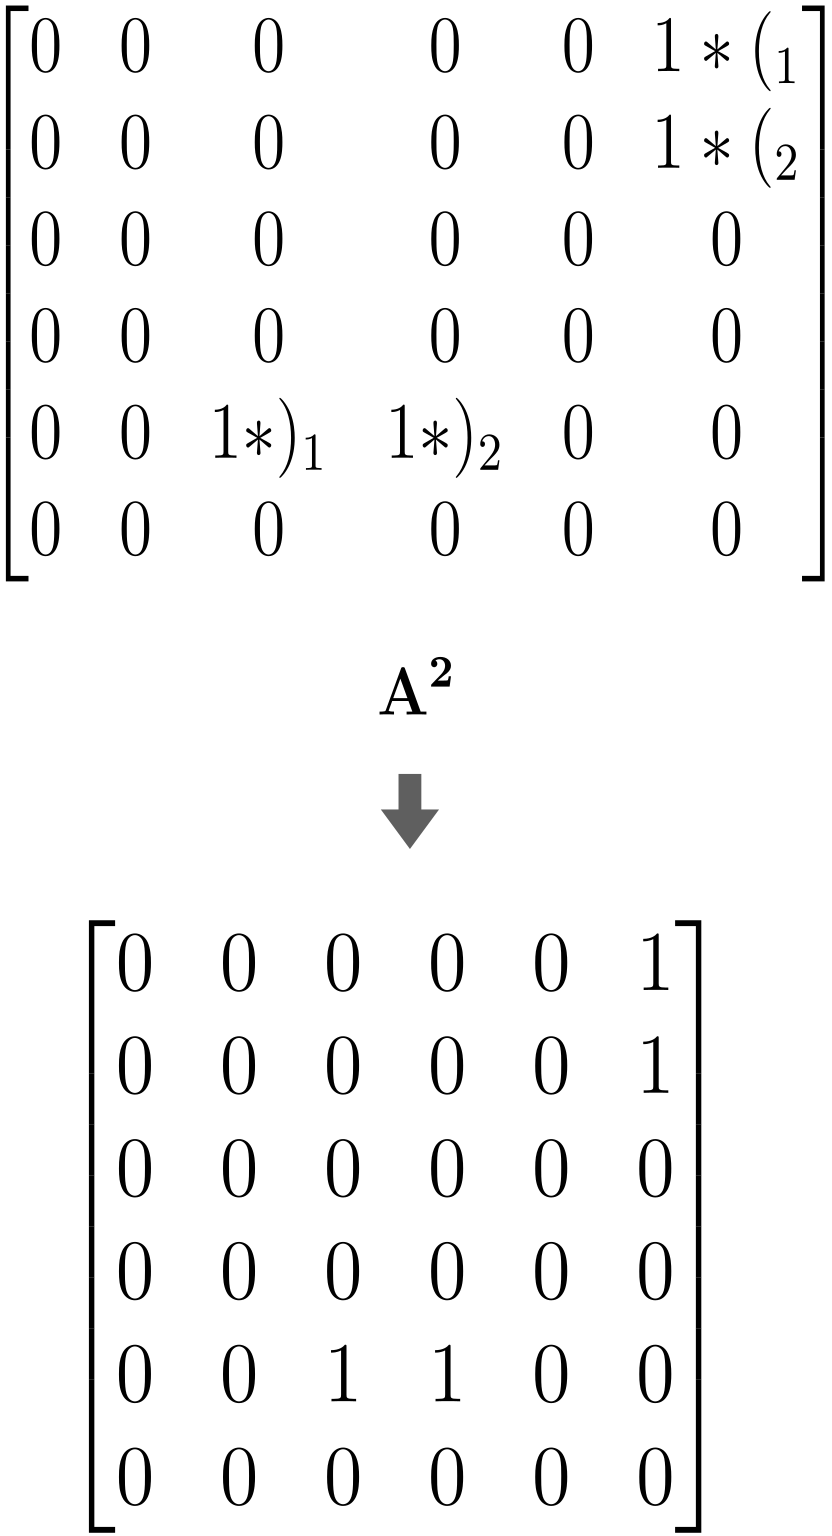
\includegraphics[width=\textwidth]{figures/cfpq_2.png}
            \caption{Matrix $A^2$}
        \end{subfigure}
        \hfill
        \begin{subfigure}[b]{0.297\textwidth}
            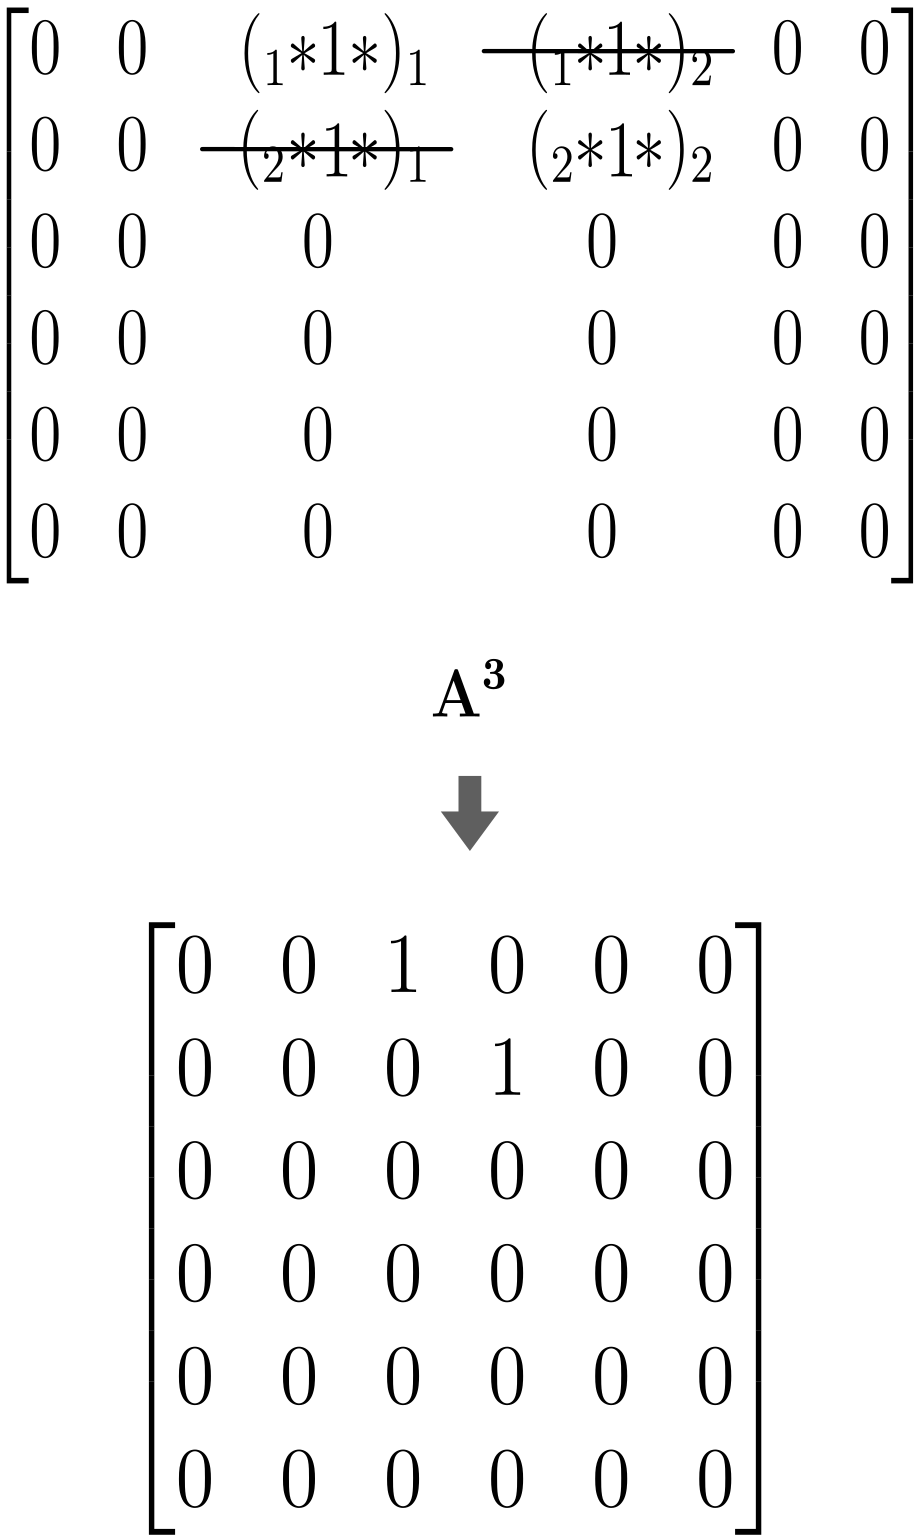
\includegraphics[width=\textwidth]{figures/cfpq_3.png}
            \caption{Matrix $A^3$}
        \end{subfigure}
        \caption{Context-sensitive value-flow reachability. $A_{ij}^h$ is the number of value-flow paths between $l_i$ and $l_j$ of length $h$.}
    \end{figure}
\end{frame}

\begin{frame}[fragile] \frametitle{Flow2vec: High-order proximity embedding}
    \begin{figure}
        \centering
        \begin{subfigure}[b]{0.38\textwidth}
            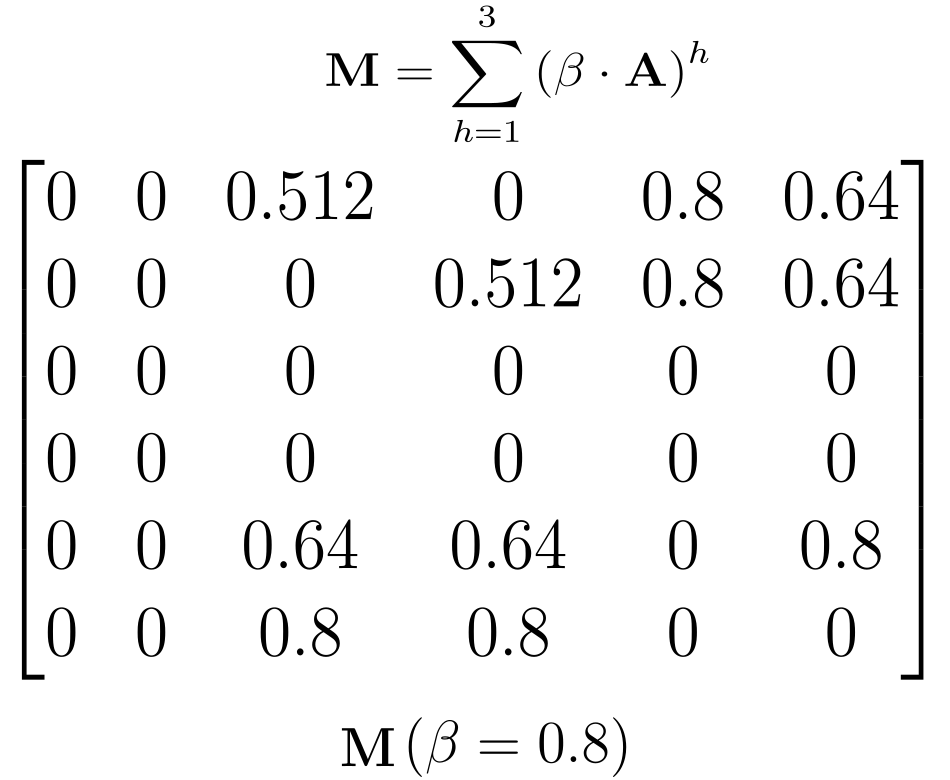
\includegraphics[width=\textwidth]{figures/proximity_matrix.png}
            \caption{High-order proximity matrix}
        \end{subfigure}
        \hfill
        \begin{subfigure}[b]{0.6\textwidth}
            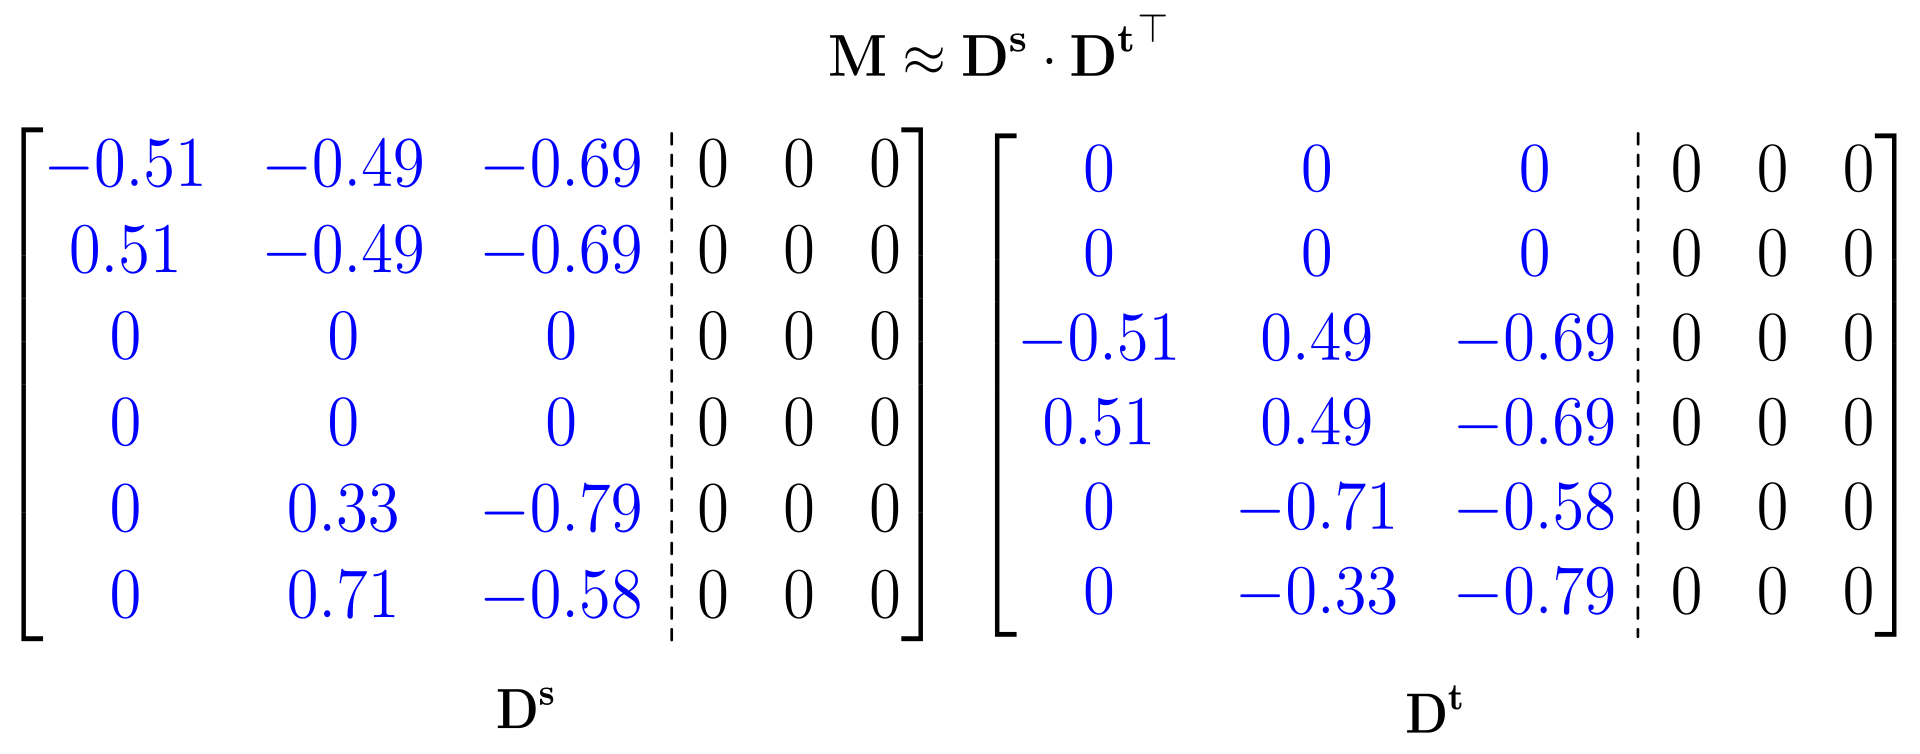
\includegraphics[width=\textwidth]{figures/embedding_vectors.png}
            \caption{Embedding vectors ($K$-factor is 3)}
        \end{subfigure}
        \caption{Embedding step}
    \end{figure}
\end{frame}

\begin{frame}[fragile] \frametitle{Flow2vec: Application scenarios}
    \begin{minipage}[m]{\linewidth}
        \begin{figure}
            \centering
            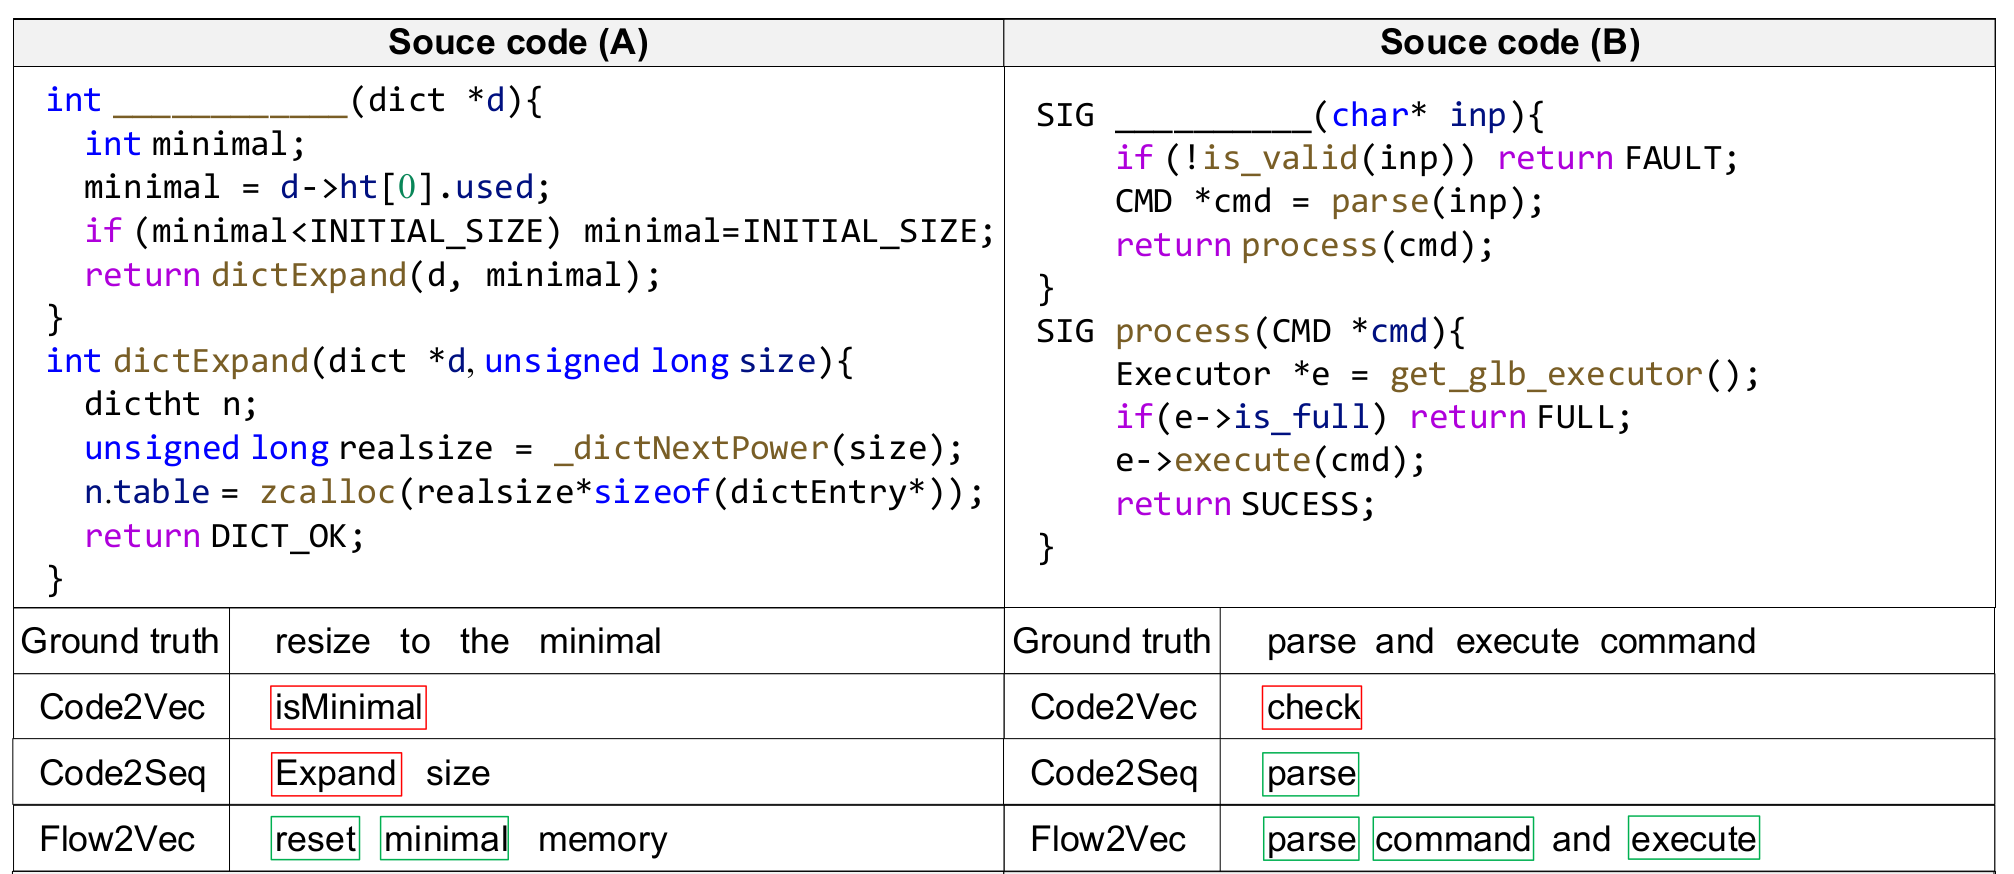
\includegraphics[width=0.7\textwidth]{figures/code_summarization_example.png}
            \caption{Code summarization example}
            \label{fig:code_summ_ex}
        \end{figure}
    \end{minipage}\hfill
    \begin{minipage}[m]{\linewidth}
        \begin{itemize}
            \item Code classification
            \item Code summarization
        \end{itemize}
    \end{minipage}
\end{frame}

\begin{frame}[fragile] \frametitle{Flow2vec: Code classification}
    \begin{itemize}
        \item Задача: предсказать метки по фрагменту кода
        \item Цель обучения: предсказывать вероятность $P(y_i~|~x)$
        \item Контекстный вектор $c_i = embedding(\langle x_i, vfp_n, x_j \rangle) = [value\_vocab_s, d_i^s \cdot {d_j^t}^T, value\_vocab_t] \in \mathbb{R}^{2d + 1}$
        \item Комбинированный контекстный вектор $\tilde{c_i} = tanh(W * c_i) \in \mathbb{R}^d$, $W \in \mathbb{R}^{d \times 2d+1}$
        \item Веса внимания $\alpha_i = \frac{exp({c_i}^T \cdot \textbf{a})}{\Sigma_{j=1}^n exp({c_j}^T \cdot \textbf{a})}$
        \item Вектор фрагмента кода $\textbf{v} = \Sigma_{i=1}^n \alpha_i \tilde{c_i}$
        \item Предсказание $y_i \in Y, q(y) = \frac{exp(\textbf{v}^T \cdot \textit{tags\_vocab}_i)}{\Sigma_{i=1}^{|Y|} exp(\textbf{v}^T \cdot \textit{tags\_vocab}_j) }$, $Y$ множество меток
    \end{itemize}
\end{frame}

\begin{frame}[fragile] \frametitle{Flow2vec: Code summarization}
    \begin{itemize}
        \item Задача: преобразовать фрагмент кода в последовательность слов 
        \item Цель обучения: предсказание вероятност $P(y_1, ..., y_m~|~x)$, $Y$ множество слов
        \item $P(y_1, ..., y_m~|~x) = \Pi_{t=1}^m P(y_t~|~y_1, ..., y_{t-1}, v)$
        \item Итеративно предсказываем каждое новое слово $y_t$ с учетом уже предсказанных $y_1, ..., y_{t-1}$
        \item С учетом механизма привлечения внимания к путям
    \end{itemize}
\end{frame}

\begin{frame}[fragile] \frametitle{Flow2vec: Резюме}
    \begin{itemize}
        \item Используя LLVM-IR, SSA форму и анализ указателей, можем строить IVFG программы
        \item Используя запросы с КС ограничениями, можем строить матрицу близости высоского порядка, которая учитывает ассиметричные потоки анных как внутри, так и между различных процедур
        \item Используя результаты работы HOPE, можем построить embedding программы
        \item Используя path-attention механизм работы code2vec, можем решать задачи обобщения и классификации кода
    \end{itemize}
\end{frame}

\begin{frame}[fragile] \frametitle{Заключение}
    \begin{itemize}
        \item Code2vec: статический анализ кода с построением embedding'а кода с использованием path-attention механизма на основе методов машинного обучения
        \item HOPE: построение embedding'а графа с сохранением ассиметричной транзитивности
        \item CFPQ: применение КС запросов для анализа графа
        \item Flow2Vec: объединение идей Code2vec, HOPE, CFPQ для построения графа потока данных программы, поиска потоков данных между всеми вершинами, построения embedding'а, и использования этого embedding'а вместе с path-attention механизмом в прикладных задачах 
    \end{itemize}
\end{frame}

% \begin{frame}[fragile] \frametitle{Kronecker CFPQ}
%     \begin{figure}
%         \centering
%         \begin{subfigure}[b]{0.2\textwidth}
%             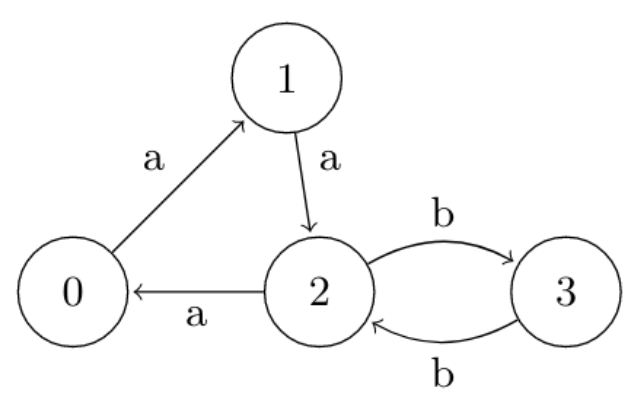
\includegraphics[width=\textwidth]{figures/graph.png}
%             \caption{Input directed graph $\mathcal{G}$}
%         \end{subfigure}
%         \hfill
%         \begin{subfigure}[b]{0.2\textwidth}
%             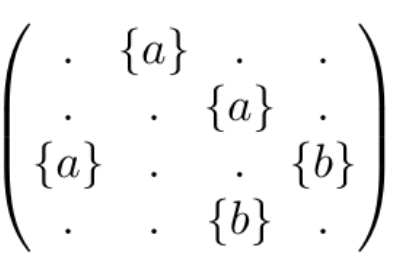
\includegraphics[width=\textwidth]{figures/graph_matrix.png}
%             \caption{$\mathcal{G}$ adjacency matrix}
%         \end{subfigure}
%         \hfill
%         \begin{subfigure}[b]{0.2\textwidth}
%             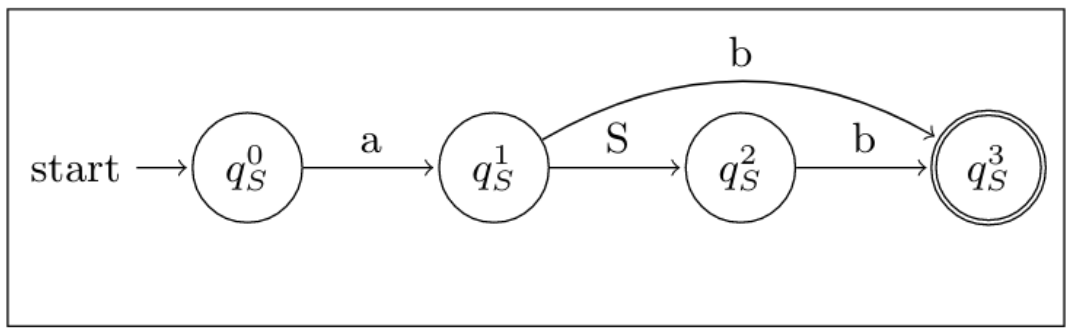
\includegraphics[width=\textwidth]{figures/automata.png}
%             \caption{RSA for $S \rightarrow ab~|~aSb$}
%         \end{subfigure}
%         \hfill
%         \begin{subfigure}[b]{0.2\textwidth}
%             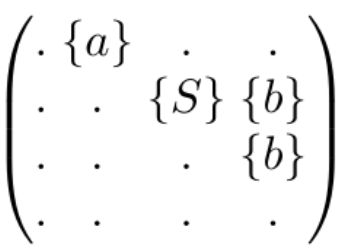
\includegraphics[width=\textwidth]{figures/automata_matrix.png}
%             \caption{RSA adjacency matrix}
%         \end{subfigure}
%         \hfill
%         \begin{subfigure}[b]{0.3\textwidth}
%             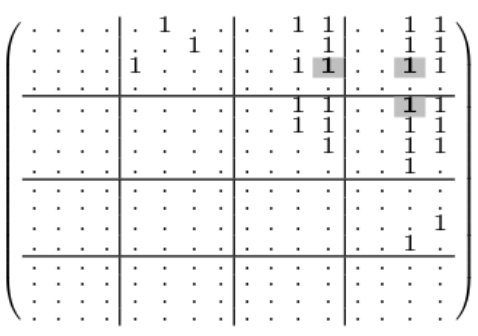
\includegraphics[width=\textwidth]{figures/kronecker_result.png}
%             \caption{Result index}
%         \end{subfigure}
%         \caption{Kronecker CFPQ brief example}
%     \end{figure}
% \end{frame}

% \begin{frame}[fragile] \frametitle{Заключение}
%     \begin{itemize}
%         \item Flow2Vec: связь анализа кода, CFPQ, и методов машинного обучения
%         \item CFPQ для всех путей
%         \item Вычисления на GPU
%         \item Что с этим делать?
%     \end{itemize}
% \end{frame}

\begin{frame} \frametitle{Дополнительно}
    \begin{itemize}
        \item Почта: \href{mailto:egororachyov@gmail.com}{egororachyov@gmail.com}
        \item Материалы презентации:
        {
            \begin{itemize}
                \item Flow2Vec: Value-Flow-Based Precise Code Embedding, Yulei Sui, Xiao Cheng, Guanqin Zhang, Haoyu Wang, \href{https://dl.acm.org/doi/10.1145/3428301}{https://dl.acm.org/doi/10.1145/3428301}
                \item Code2vec: learning distributed representations of code, Uri Alon, Meital Zilberstein, Omer Levy, and Eran Yahav, \href{https://doi.org/10.1145/3290353}{https://doi.org/10.1145/3290353}
                \item Asymmetric Transitivity Preserving Graph Embedding, Mingdong Ou, Peng Cui, Jian Pei, Ziwei Zhang, and Wenwu Zhu, \href{https://doi.org/10.1145/2939672.2939751}{https://doi.org/10.1145/2939672.2939751}
                \item Context-Free Path Querying with Single-Path Semantics by Matrix Multiplication, Arseniy Terekhov, Artyom  Khoroshev, Rustam  Azimov, Semyon Grigorev, \href{https://dl.acm.org/doi/10.1145/3398682.3399163}{https://dl.acm.org/doi/10.1145/3398682.3399163}
                \item Context-Free Path Querying by Kronecker Product, Egor Orachev, Ilya Epelbaum, Rustam  Azimov, Semyon Grigorev, \href{https://link.springer.com/chapter/10.1007/978-3-030-54832-2\_6}{https://link.springer.com/chapter/10.1007/978-3-030-54832-2\_6}
            \end{itemize}
        }
    \end{itemize}
\end{frame}

\end{document}
